\documentclass{article}
\usepackage{graphicx}
\usepackage{amsmath}% http://ctan.org/pkg/amsmath
\usepackage{kbordermatrix}% http://www.hss.caltech.edu/~kcb/TeX/kbordermatrix.sty

\usepackage[L7x,T2A]{fontenc}
\usepackage[utf8]{inputenc}
\usepackage[lithuanian]{babel}

\usepackage{breqn}
\usepackage{mathtools,hyperref}
\usepackage{float}







\usepackage{caption}

\usepackage{subcaption}

\begin{document}

\title{Natural Language Processing for Lithuanian language}
\author{Mindaugas Venckus}

\maketitle
The main intention of this research is to study and learn natural language processing (NLP) principals  for Lithuanian language. It is interesting to analyze classical NLP methods and see how they work on it, so in this work I implemented text classification, topics extraction, search query and clustering ideas.
\begin{abstract}

\end{abstract}

\section{Data}
Data analysis can't be established without having textual data, due to that my work started from getting raw data from most popular news website www.delfi.lt. I decided to crawl articles from 5 categories (Criminals, Music, Movies, Sports, Science) such approach helps me to understand the performance of NLP methods better. Below basic statistics of data that was analyzed is presented  \ref{DocumentsTable}.
\begin{table}[htb]
\centering
\caption{Documents}
\label{DocumentsTable}
\begin{tabular}{|l|l|}
\hline
          & documents count \\ \hline
criminals & 227             \\ \hline
movies    & 167             \\ \hline
music     & 120             \\ \hline
science   & 204             \\ \hline
sports    & 136             \\ \hline
\end{tabular}
\end{table}
\section{Preprocessing}
 
At first we need to convert unstructured data (raw text) to structured (matrix based approach) -  such transformation is friendly for machine learning algorithms. Preprocessing goal is to convert unstructured data to  structured matrix where rows are document id, columns - token, values - term frequency inverse document frequency (TFIDF) statistic.


\renewcommand{\kbldelim}{(}% Left delimiter
\renewcommand{\kbrdelim}{)}% Right delimiter
\[
  \text{tfidf\_matrix} = \kbordermatrix{
    & token_1 & token_2 & token_3 & . & token_n \\
    doc_1 & 0 & 0 &  & . & 0 \\
    doc_2 & 0 &  & 0.14 & . & 0 \\
    doc_3 & 0 & 0 & 0 & . & 0 \\
    . & . & . & . & . & . \\
    doc_n & 0 & 0.011 & 0 & . & 0
  }
\]

\subsection{Tokenization}
Suppose we have the sample of raw text bellow: \\
\textsc{Pranešimas gautas apie 14.14 val. Kaune, Švenčionių g. prie Nemuno upės ant kranto rastas žmogaus kūnas su galimai durtine žaizda krūtinėje. Aplinkybės tikslinamos.}
Tokenization is the process of breaking a text into smaller words, phrases and symbols. In this case we are trying to break text into the words.

\begin{enumerate}
\item  Break text into the words using regex expression \text{W+} which breaks text by any non-word character.
\begin{enumerate}
\item Remove digits
\item Remove words smaller than 4 letters
\item Remove stop words (unnecessary/common words)
\item Remove word endings
\end{enumerate}
\end{enumerate}
Text above is transformed to list representation
\textsc{t = [aplinkyb, durtin, gaut, kaun, krant, krūtin, kūn, nemun, praneš, rast, tikslinam, up ,švenčion, žaizd, žmog]}


\subsection{TFIDF}
TFIDF \ref{tfidf} is statistic which measure token importance in document with relation to the document of corpus.
\begin{equation}
\label{tfidf}
tfidf(t, d, D) = tf(t, d) \cdot  idf(t,D)
\end{equation}

where term frequency $ tf(t, d)$  is a measure of how many times token $t$ occurs in the document $d$ and inverse document frequency $idf(t, D) $ is a measure of how much information the word provides, that is, whether the term is common or rare across all documents.
\begin{equation}
idf(t, D) = \log \frac{N}{|d\in D : t \in d|}
\label{idf}
\end{equation}
with 
\begin{enumerate}
\item $N$ - total number of documents in corpus $N = |D|$
\item $|d\in D : t \in d|$ - number of documents where term $t$ appears.
\end{enumerate}
TFIDF intuitive explanation -  importance increases proportionally to the number of times a word appears in the document but is offset by the frequency of the word in the corpus.

\subsection{TFIDF matrix construction}
Main steps before TFIDF matrix construction are:
\begin{enumerate}
\item For each document $90\%$ - train set, $10\%$ - test set.
\begin{enumerate}
\item Collect tokens for each document separately.
\item Collect unique tokens.
\item Collect document categories (will be used for classification performance measuring)
\item Collect document titles (will be used for clustering)
\end{enumerate}
\end{enumerate}

TFIDF matrix rows are all documents and columns unique tokens filled with  TFIDF statistic. Additionally we reduce matrix dimension by removing tokens (entire column) which appears among documents rarely, more precisely  once a time.
\section{Classification}
Main idea of classification is to convert unseen text to vectorized token representations where tokens are taken from TFIDF matrix and do multiplication between vector and mentioned matrix. After that use k-nearest neighbors approach to make prediction for unseen document by taking mode of most similar $k$ documents categories.


\subsection{Classification results}
Classification performance is measured using confusion matrix where rows are true category and columns predicted category. The  Figure \ref{confusion matrix} shows the results of categories prediction. For example  for 21 movies  got 1 criminals, 1 science and 19 movies predictions. In overall such approach reach above $90 \%$  recall and $90 \%$ precision.
\begin{figure}[H]
  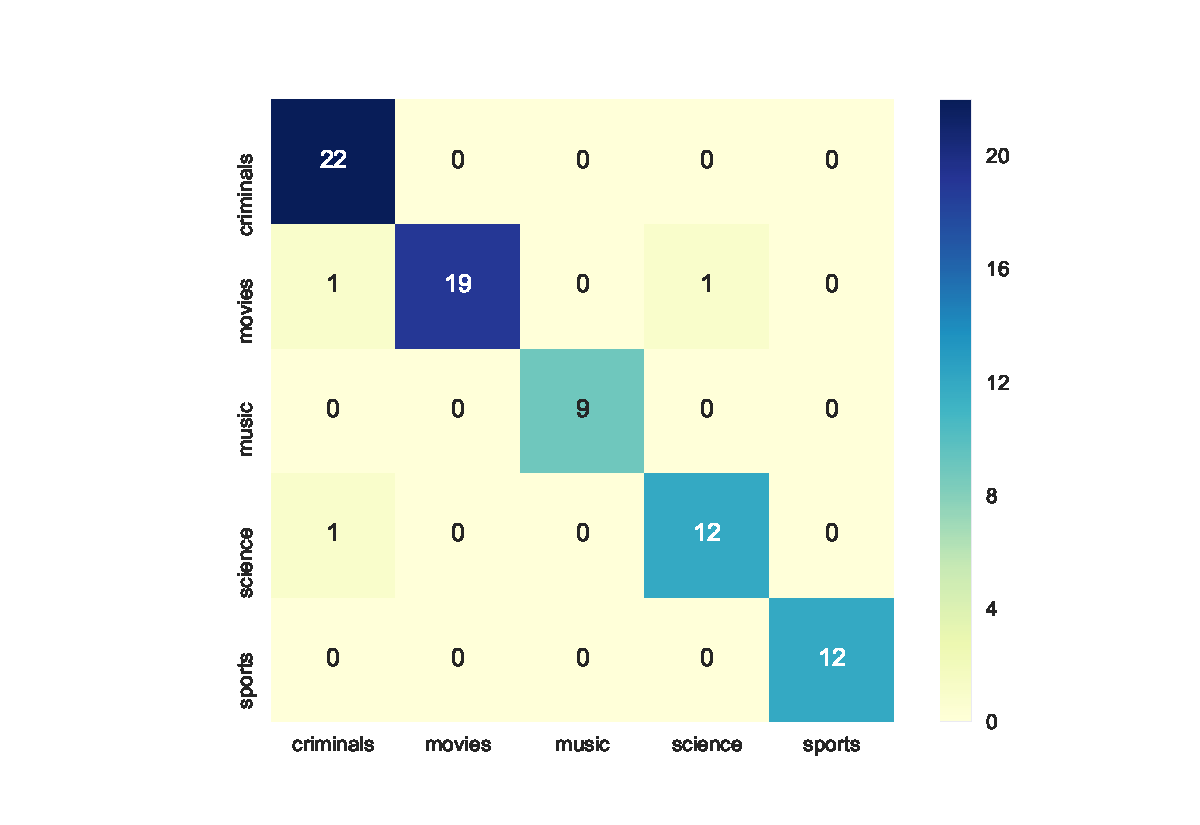
\includegraphics[width=\linewidth]{images/confussion_matrix.pdf}
  \caption{Classification performance}
  \label{confusion matrix}
\end{figure}

\section{Topics extraction}
Latent semantic analysis (LSA) is a technique in natural language processing, in particular distributional semantics, of analyzing relationships between a set of documents and the terms they contain by producing a set of concepts related to the documents and terms. Let's mark tfidf matrix as $X$, after applying singular value decomposition (SVD) we get 
\begin{equation}
\label{LSA}
A =U\Sigma V^T
\end{equation}
Let $A$ be a $m \times n$ matrix with column vectors $a_1, a_2, ..., a_n$. In the SVD of, U will be $m \times m$, $\Sigma$ will be $m \times n$ and $V$ will be $n \times n$. Dimensionality reduction is done by keeping  $k$ biggest  values from $\Sigma$ i.e $\sigma_1,..,\sigma_k \neq 0$; $\sigma_{r+1},...,\sigma_n = 0$. Therefore columns of $U$ beyond $k^{th}$ column and rows of V beyond $k^{th}$ row do not contribute to A and are usually omitted, leaving U an  $m \times k$ matrix, $\Sigma$ and  $k \times k$ diagonal matrix and $V$ an  $r \times n$ matrix. After that terms are represented by the row vectors of the $m \times k$ matrix \ref{hiddenterms}

\begin{equation}
\label{hiddenterms}
Q = U_k\Sigma_k
\end{equation}
whereas the documents by the column vectors the $k \times n$ matrix \ref{hiddendocs}
 \begin{equation}
\label{hiddendocs}
W =\Sigma_kV_k^T
\end{equation}

Topics can represented as rows from matrix $U^T$ $(k \times m)$, where rows are principal components, columns are tokens. 
\begin{enumerate}
\item Extract first $x$ rows (components).
\item Sort each row weights in descending order.
\item Extract first $y$ highest weights and map them to the tokens we know.
\end{enumerate}


 Results figure \ref{main_terms_components} shows $6$ components with $10$ tokens for each component. From these results we can detect most important words and intuitively guess topic for each principal component. For example 3 principal component store information about  sports and music whereas 5 principal component store information about criminals.


\begin{figure}[H]
  \centering
  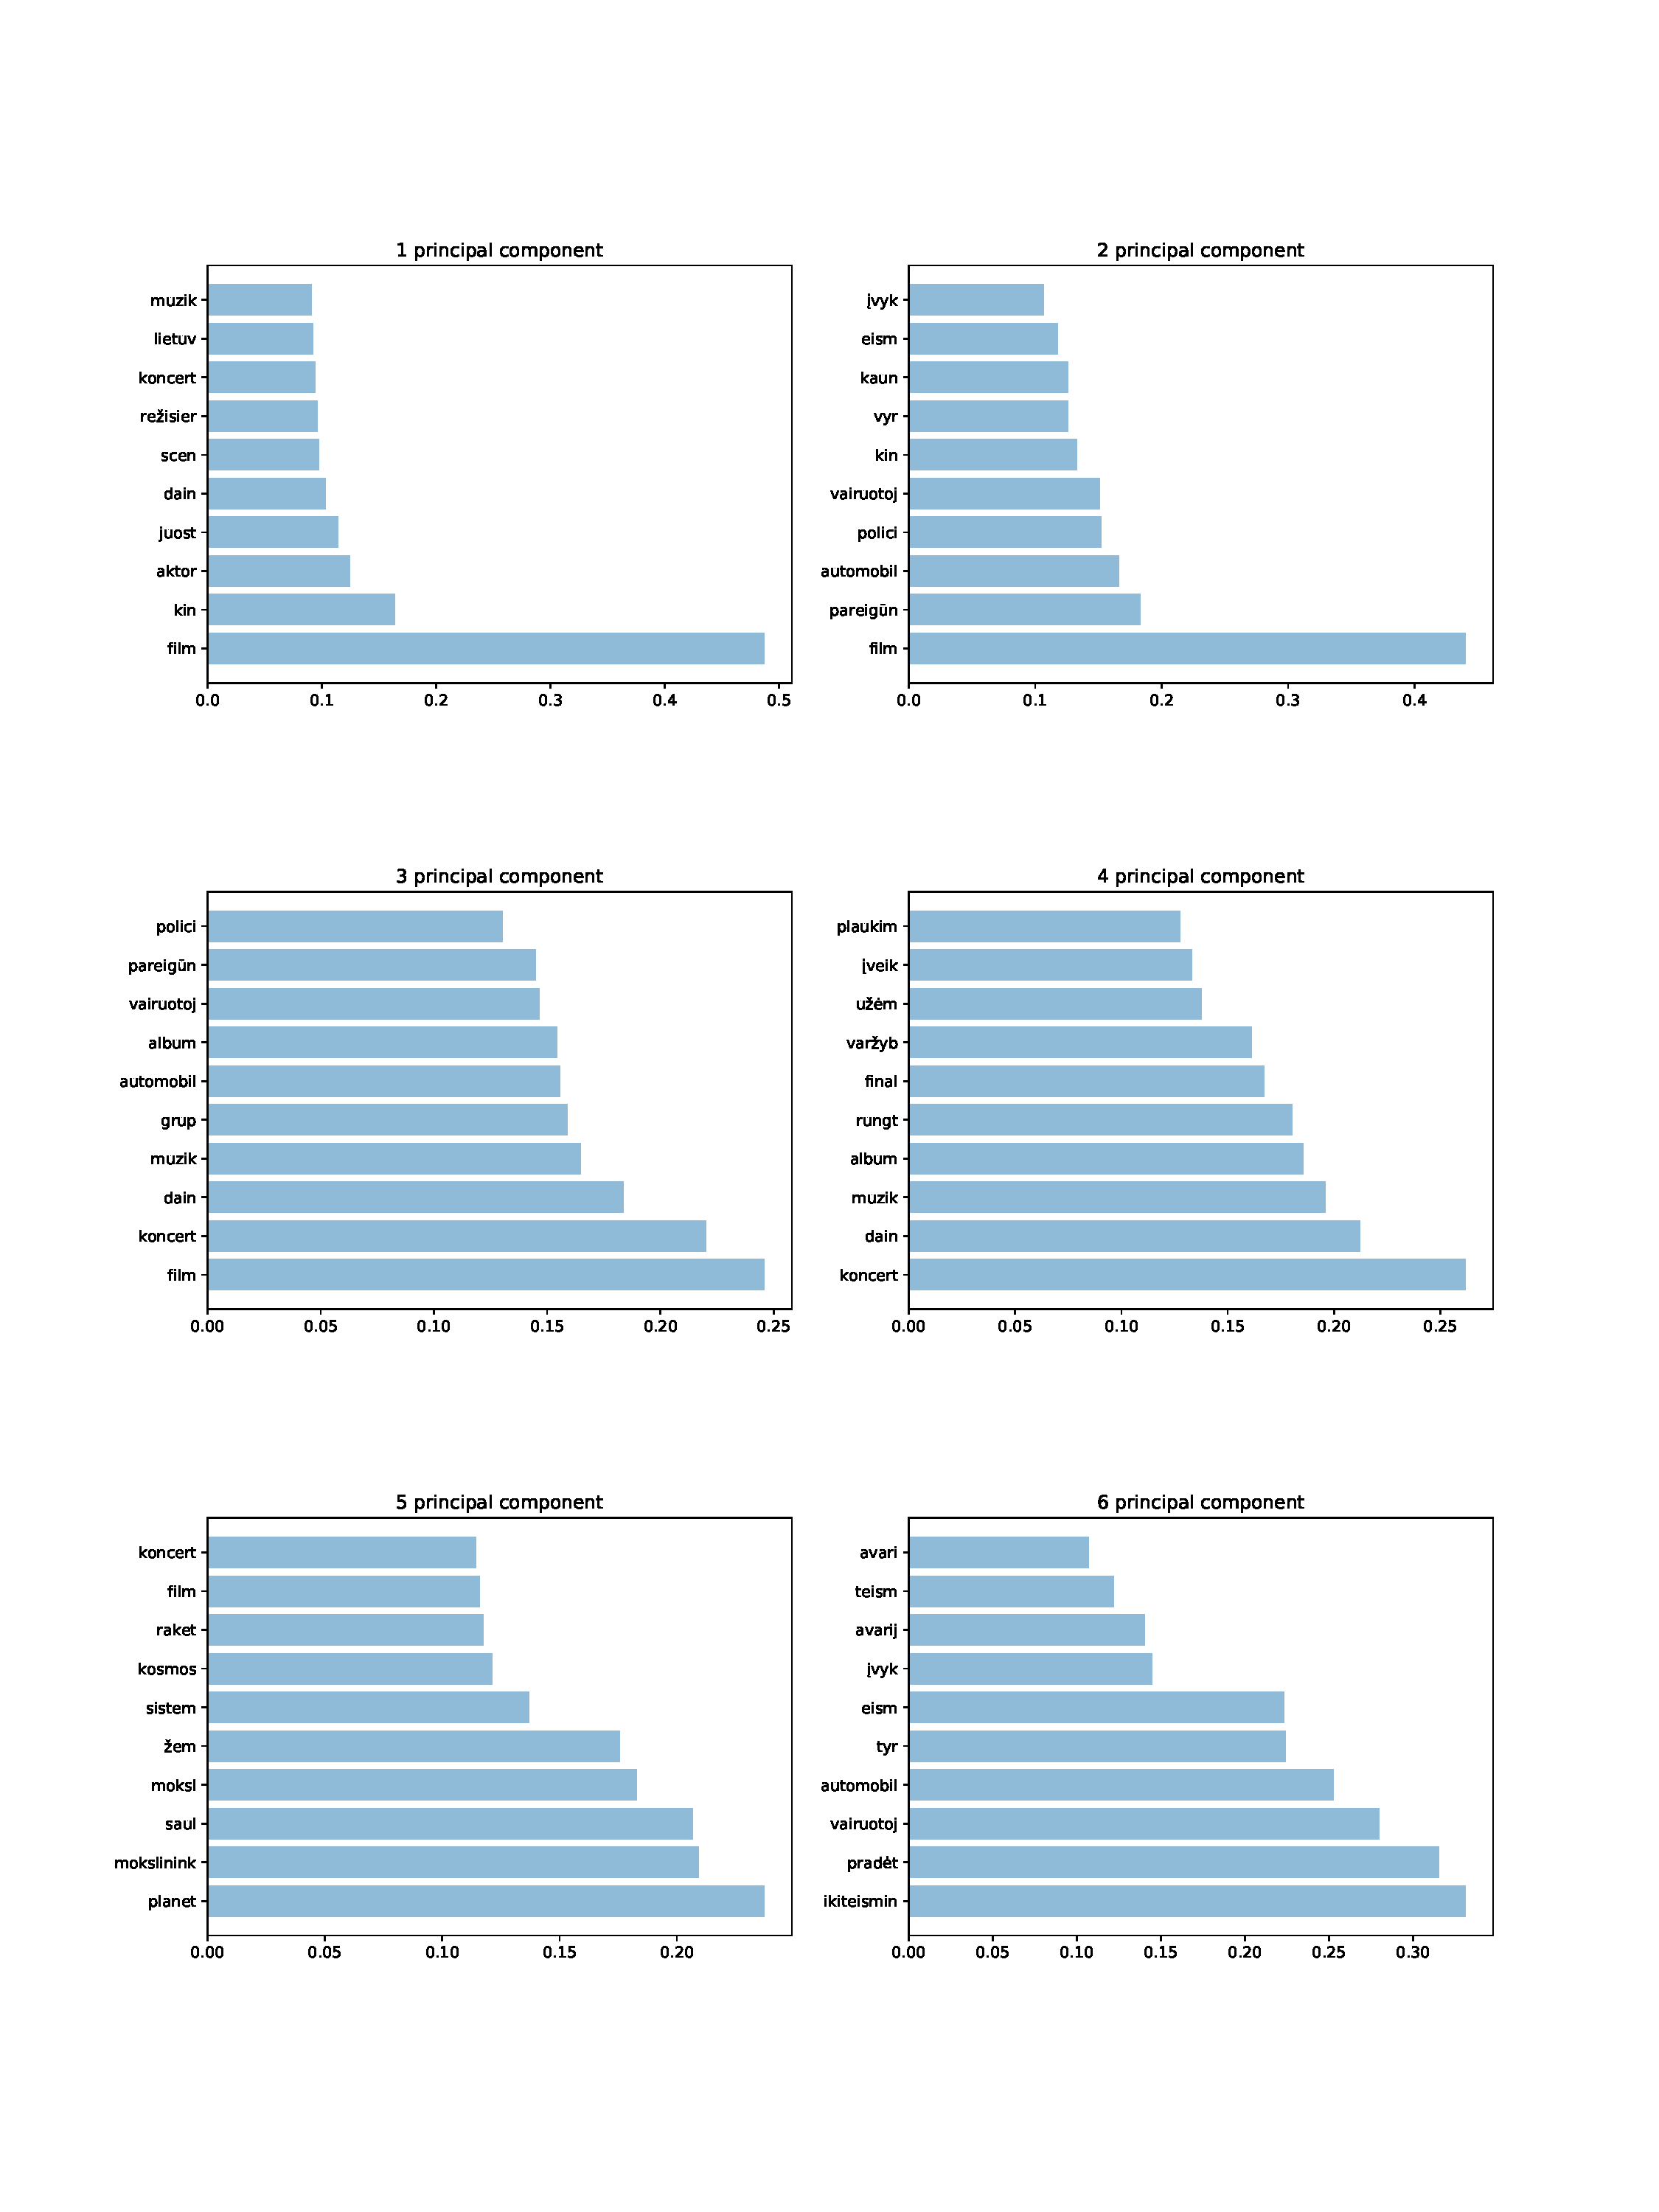
\includegraphics[scale=0.4]{images/main_term_components.pdf}
  \caption{Main term components}
  \label{main_terms_components}
\end{figure}




\end{document}